\subsection{Dealing with continuous variables}
So far we mainly assumed categorical features, for both the descriptive and target features. Now, we also want to take a look at how to deal with continuous features. Remember, that generally continuous features can be tuned into categorical ones using binning.

First, let's look at \textbf{continuous descriptive features}. The challenge is to determine suitable boundaries, where also an infinite number of thresholds is possible. The approach is:
\begin{itemize}
  \item Sort the instances based on the continuous feature and then look for changes in class labels.
  \item Points where class label changes happen are candidate thresholds.
  \item The threshold with the highest information gain is selected.
\end{itemize}

How this works is visualized as an example in \ref{fig:3_cont_descriptive_feature}.

\begin{figure}[H]
  \centering
  \begin{subfigure}{0.4\textwidth}
    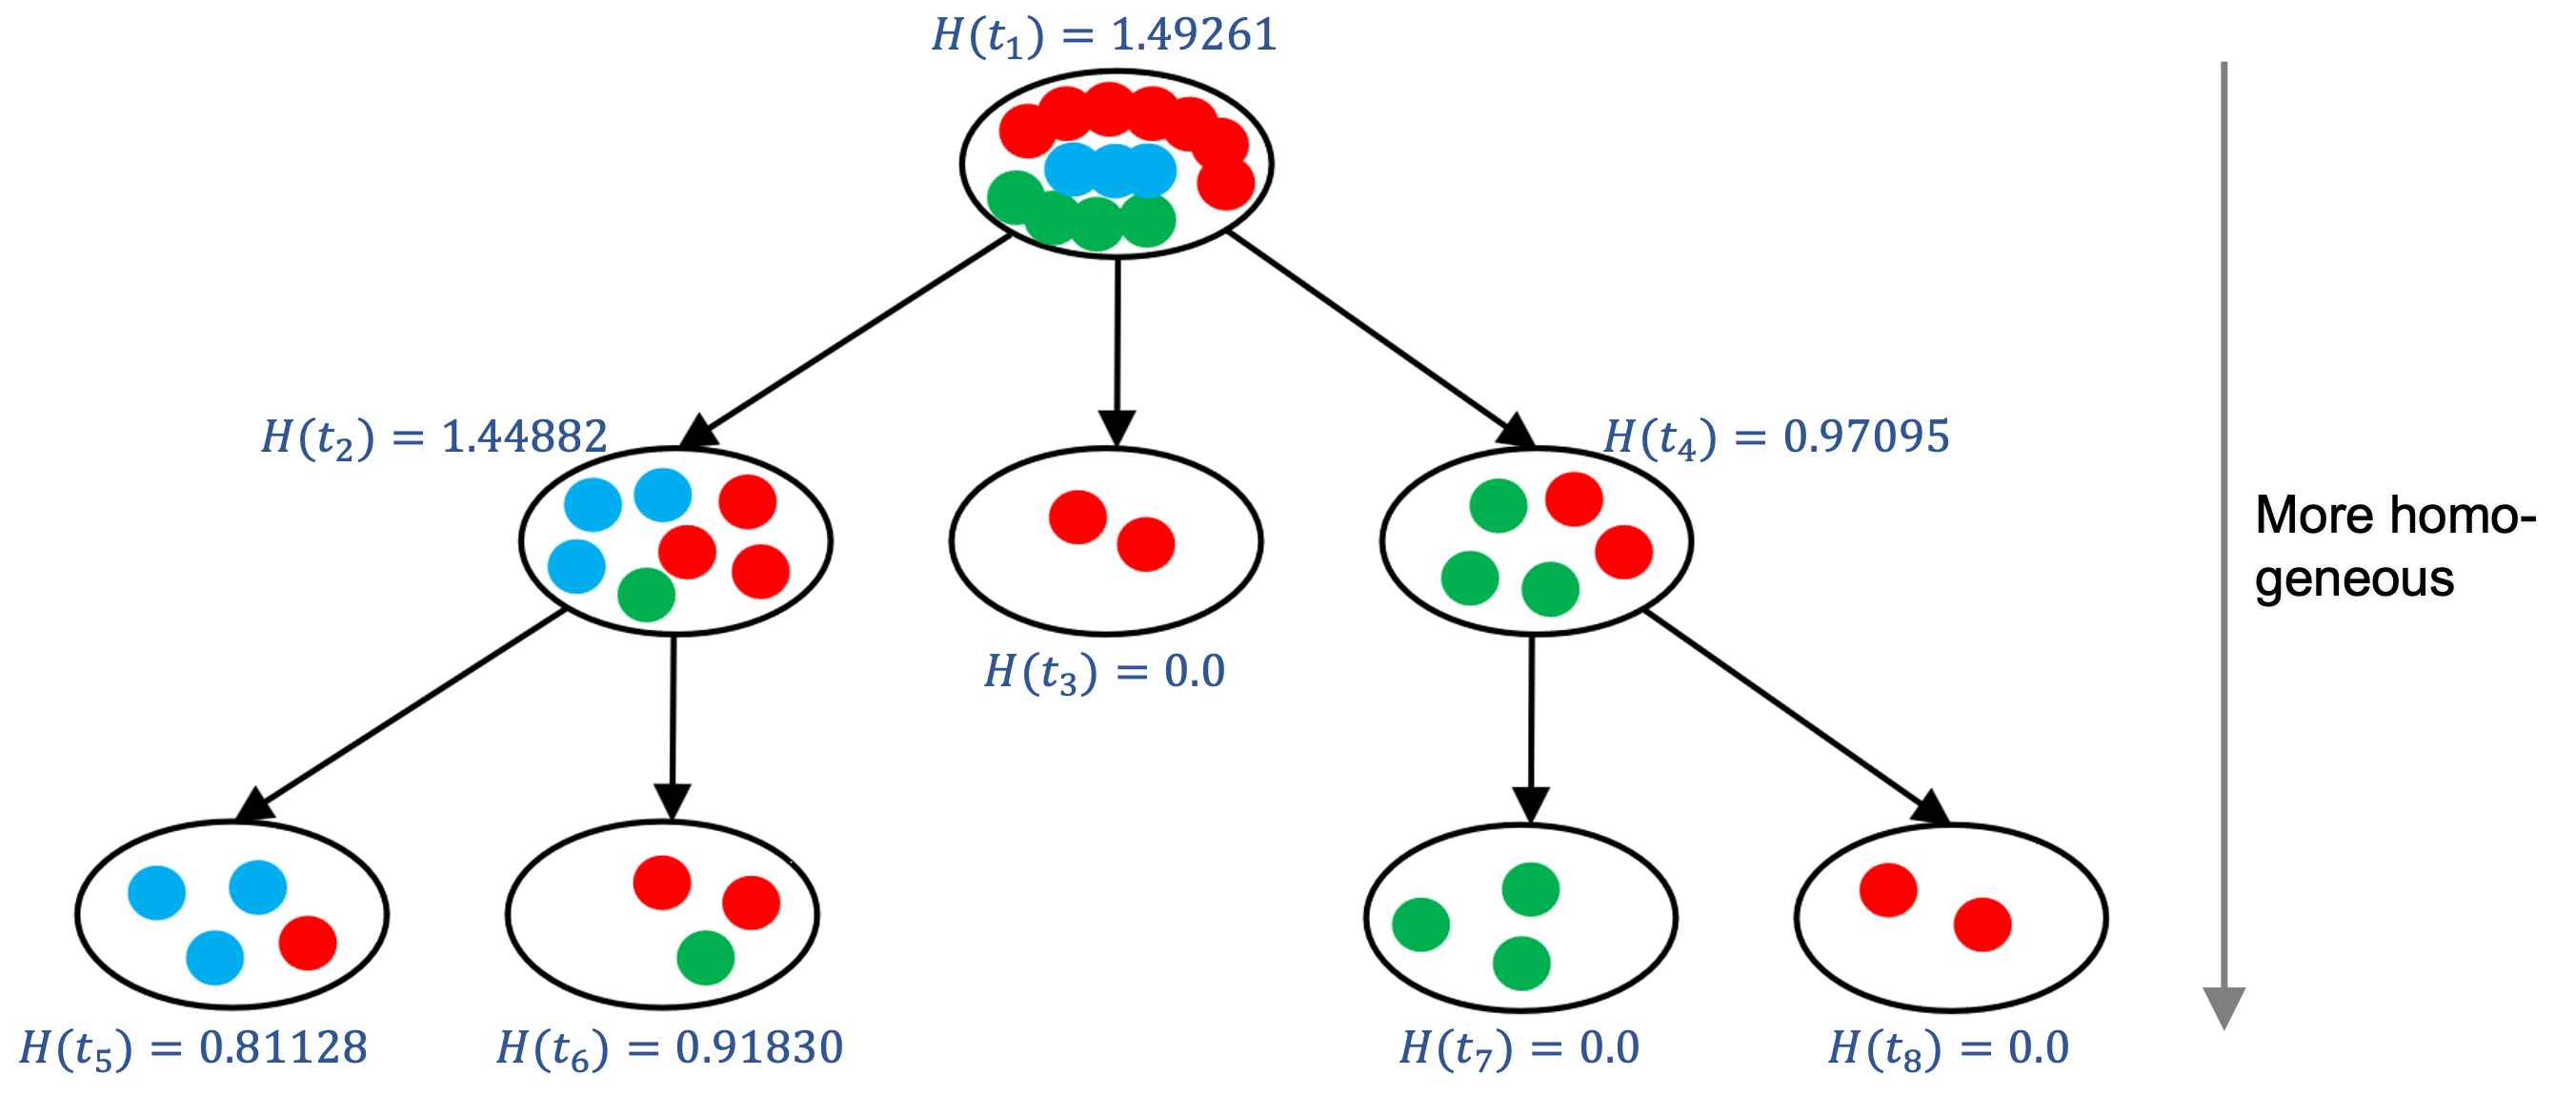
\includegraphics[width=0.8\textwidth]{assets/trees/cont/descriptive_possible.png}
    \subcaption{Possible thresholds}

    \vspace*{0.5cm}
    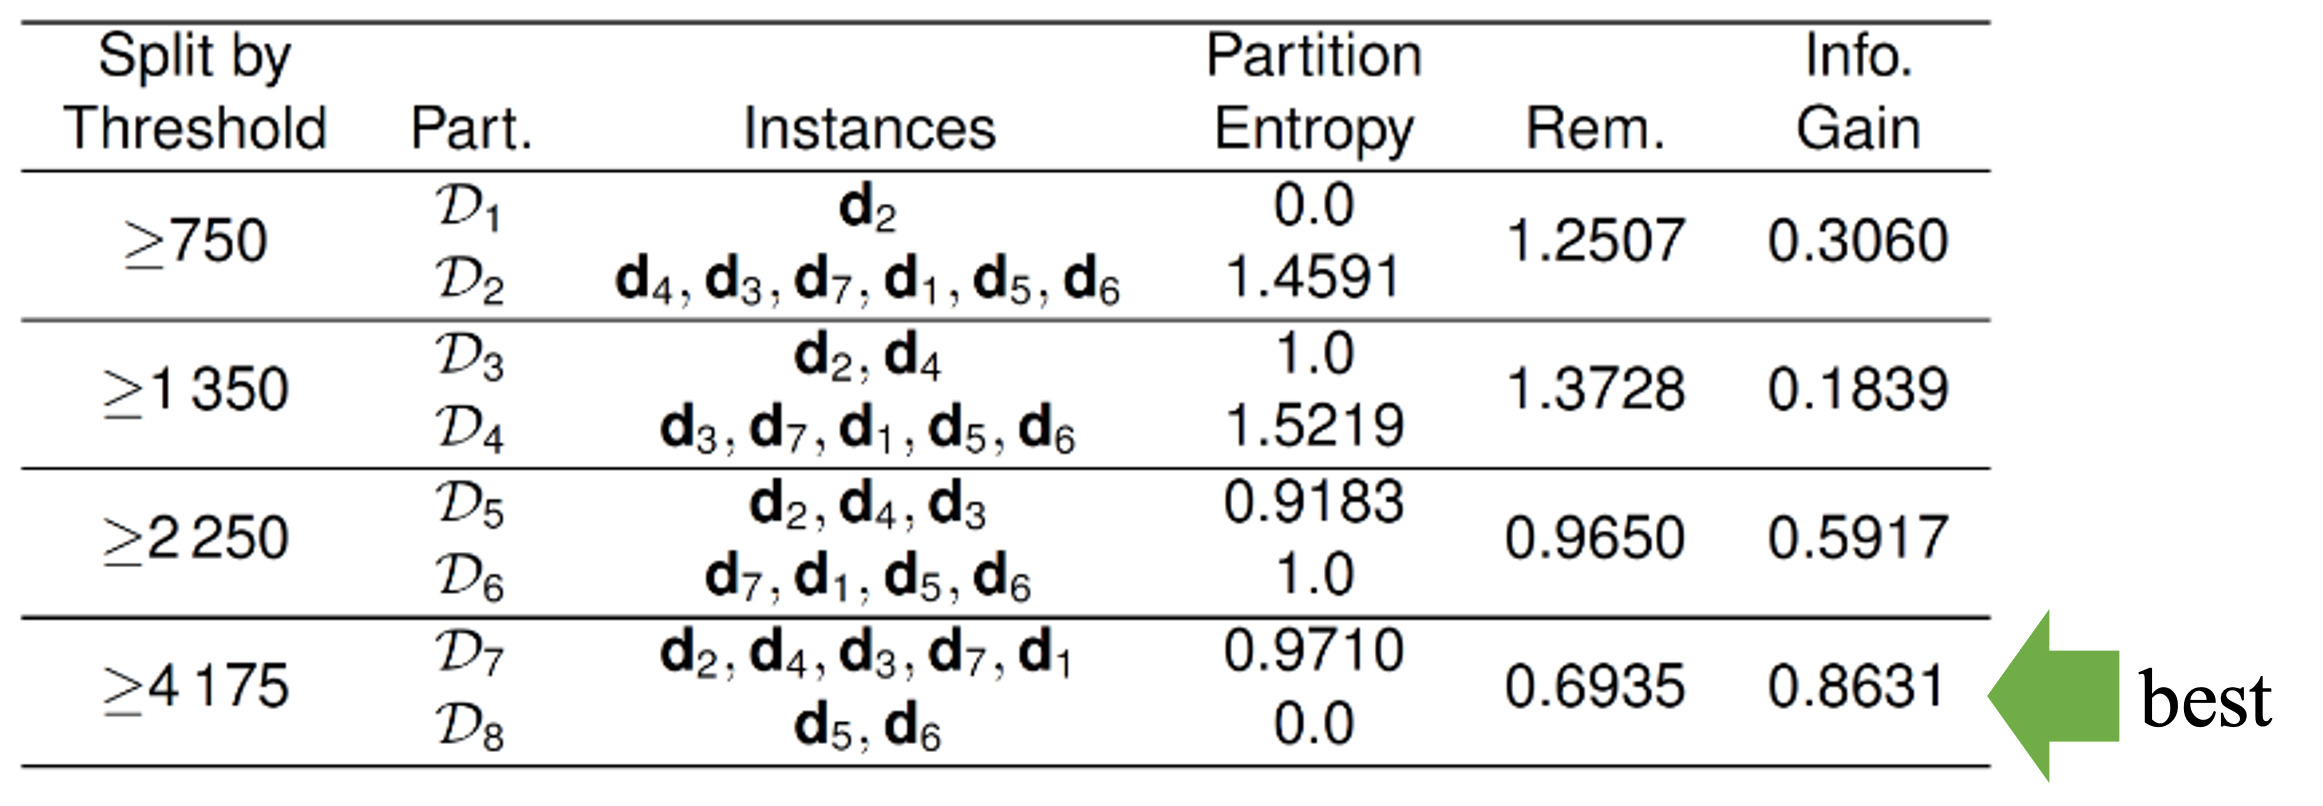
\includegraphics[width=0.9\textwidth]{assets/trees/cont/descriptive_decision.png}
    \subcaption{Thresholds selection}
  \end{subfigure}
  \begin{subfigure}{0.5\textwidth}
    \centering
    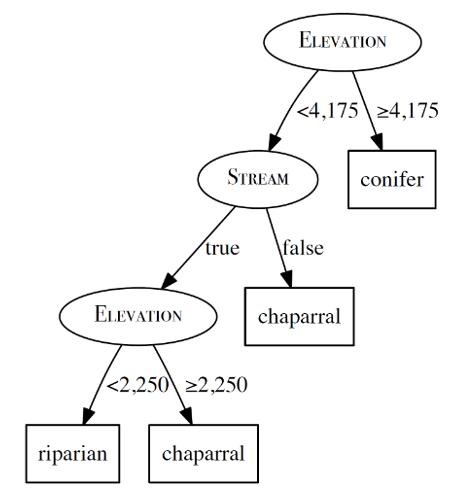
\includegraphics[width=0.6\textwidth]{assets/trees/cont/descriptive_final_trees.png}
    \subcaption{Final tree}
    \textcolor{black}{\footnotesize Note: the same feature can be used twice along a path.}
  \end{subfigure}
  \caption{Building a decision tree with a continuous descriptive feature}
  \label{fig:3_cont_descriptive_feature}
\end{figure}


Next, consider a \textbf{continuous target feature}. Here, we want to find descriptive features that "nicely" partition the target feature axis. 
\begin{itemize}
  \item How to distinguish and evaluate different classifications can be seen in \ref{fig:3_classifications_target}
  \item Impurity is measured by the variance within a partition (so a leaf in the decision tree). 
  \item But the split can't use the target feature as a decision. Instead, the weighted variance after the split is used as a performance criterion.
  \begin{itemize}
    \item The smaller, the better.
    \item $var(t, \mathcal{D}) = \frac{1}{n-1} \sum_{i=1}^{n}(\,t_i-\bar{t}\,)^2$
  \end{itemize}
\end{itemize}

\begin{figure}[h]
  \centering
  
  \begin{subfigure}{0.6\textwidth}
    \centering
    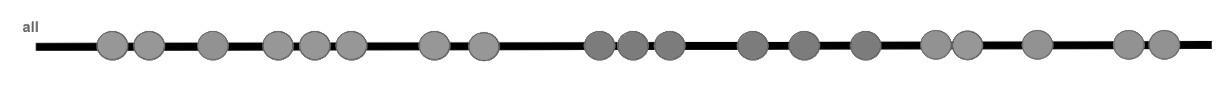
\includegraphics[width=0.9\textwidth]{assets/trees/cont/target_ori_set.png}
    \subcaption{Original dataset}
  \end{subfigure}

  \vspace*{0.5cm}
  \begin{subfigure}{0.6\textwidth}
    \centering
    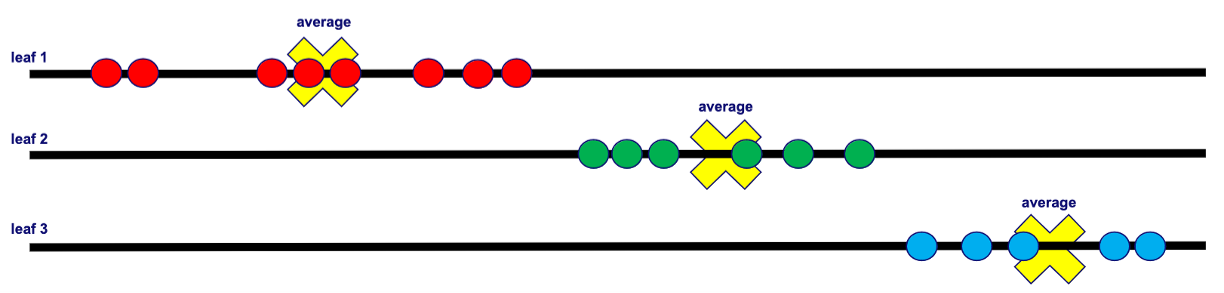
\includegraphics[width=0.9\textwidth]{assets/trees/cont/target_good.png}
    \subcaption{Good classification}
  \end{subfigure}

  \vspace*{0.5cm}
  \begin{subfigure}{0.6\textwidth}
    \centering
    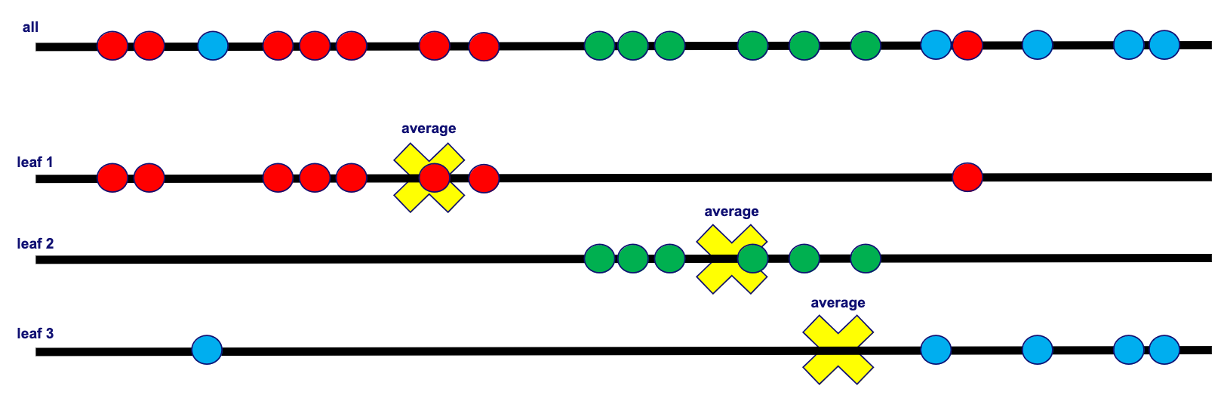
\includegraphics[width=0.9\textwidth]{assets/trees/cont/target_ok.png}
    \subcaption{Reasonable classification}
  \end{subfigure}

  \vspace*{0.5cm}
  \begin{subfigure}{0.6\textwidth}
    \centering
    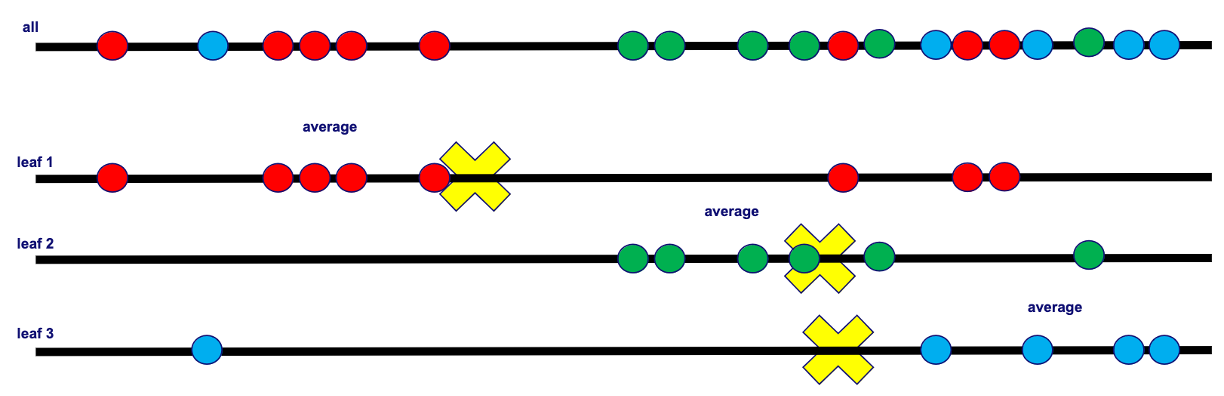
\includegraphics[width=0.9\textwidth]{assets/trees/cont/target_bad.png}
    \subcaption{Poor classification}
  \end{subfigure}
  \caption{Level of validity of different classifications for a continuous target feature}
  \label{fig:3_classifications_target}
\end{figure}

It's important to keep track of over- and underfitting, as visualized in \ref{fig:3_overunder_target}. Generally, variance gets smaller when the sets get smaller, so the measure leans towards overfitting. This can be avoided by stopping early enough.

\begin{figure}[h]
  \centering
  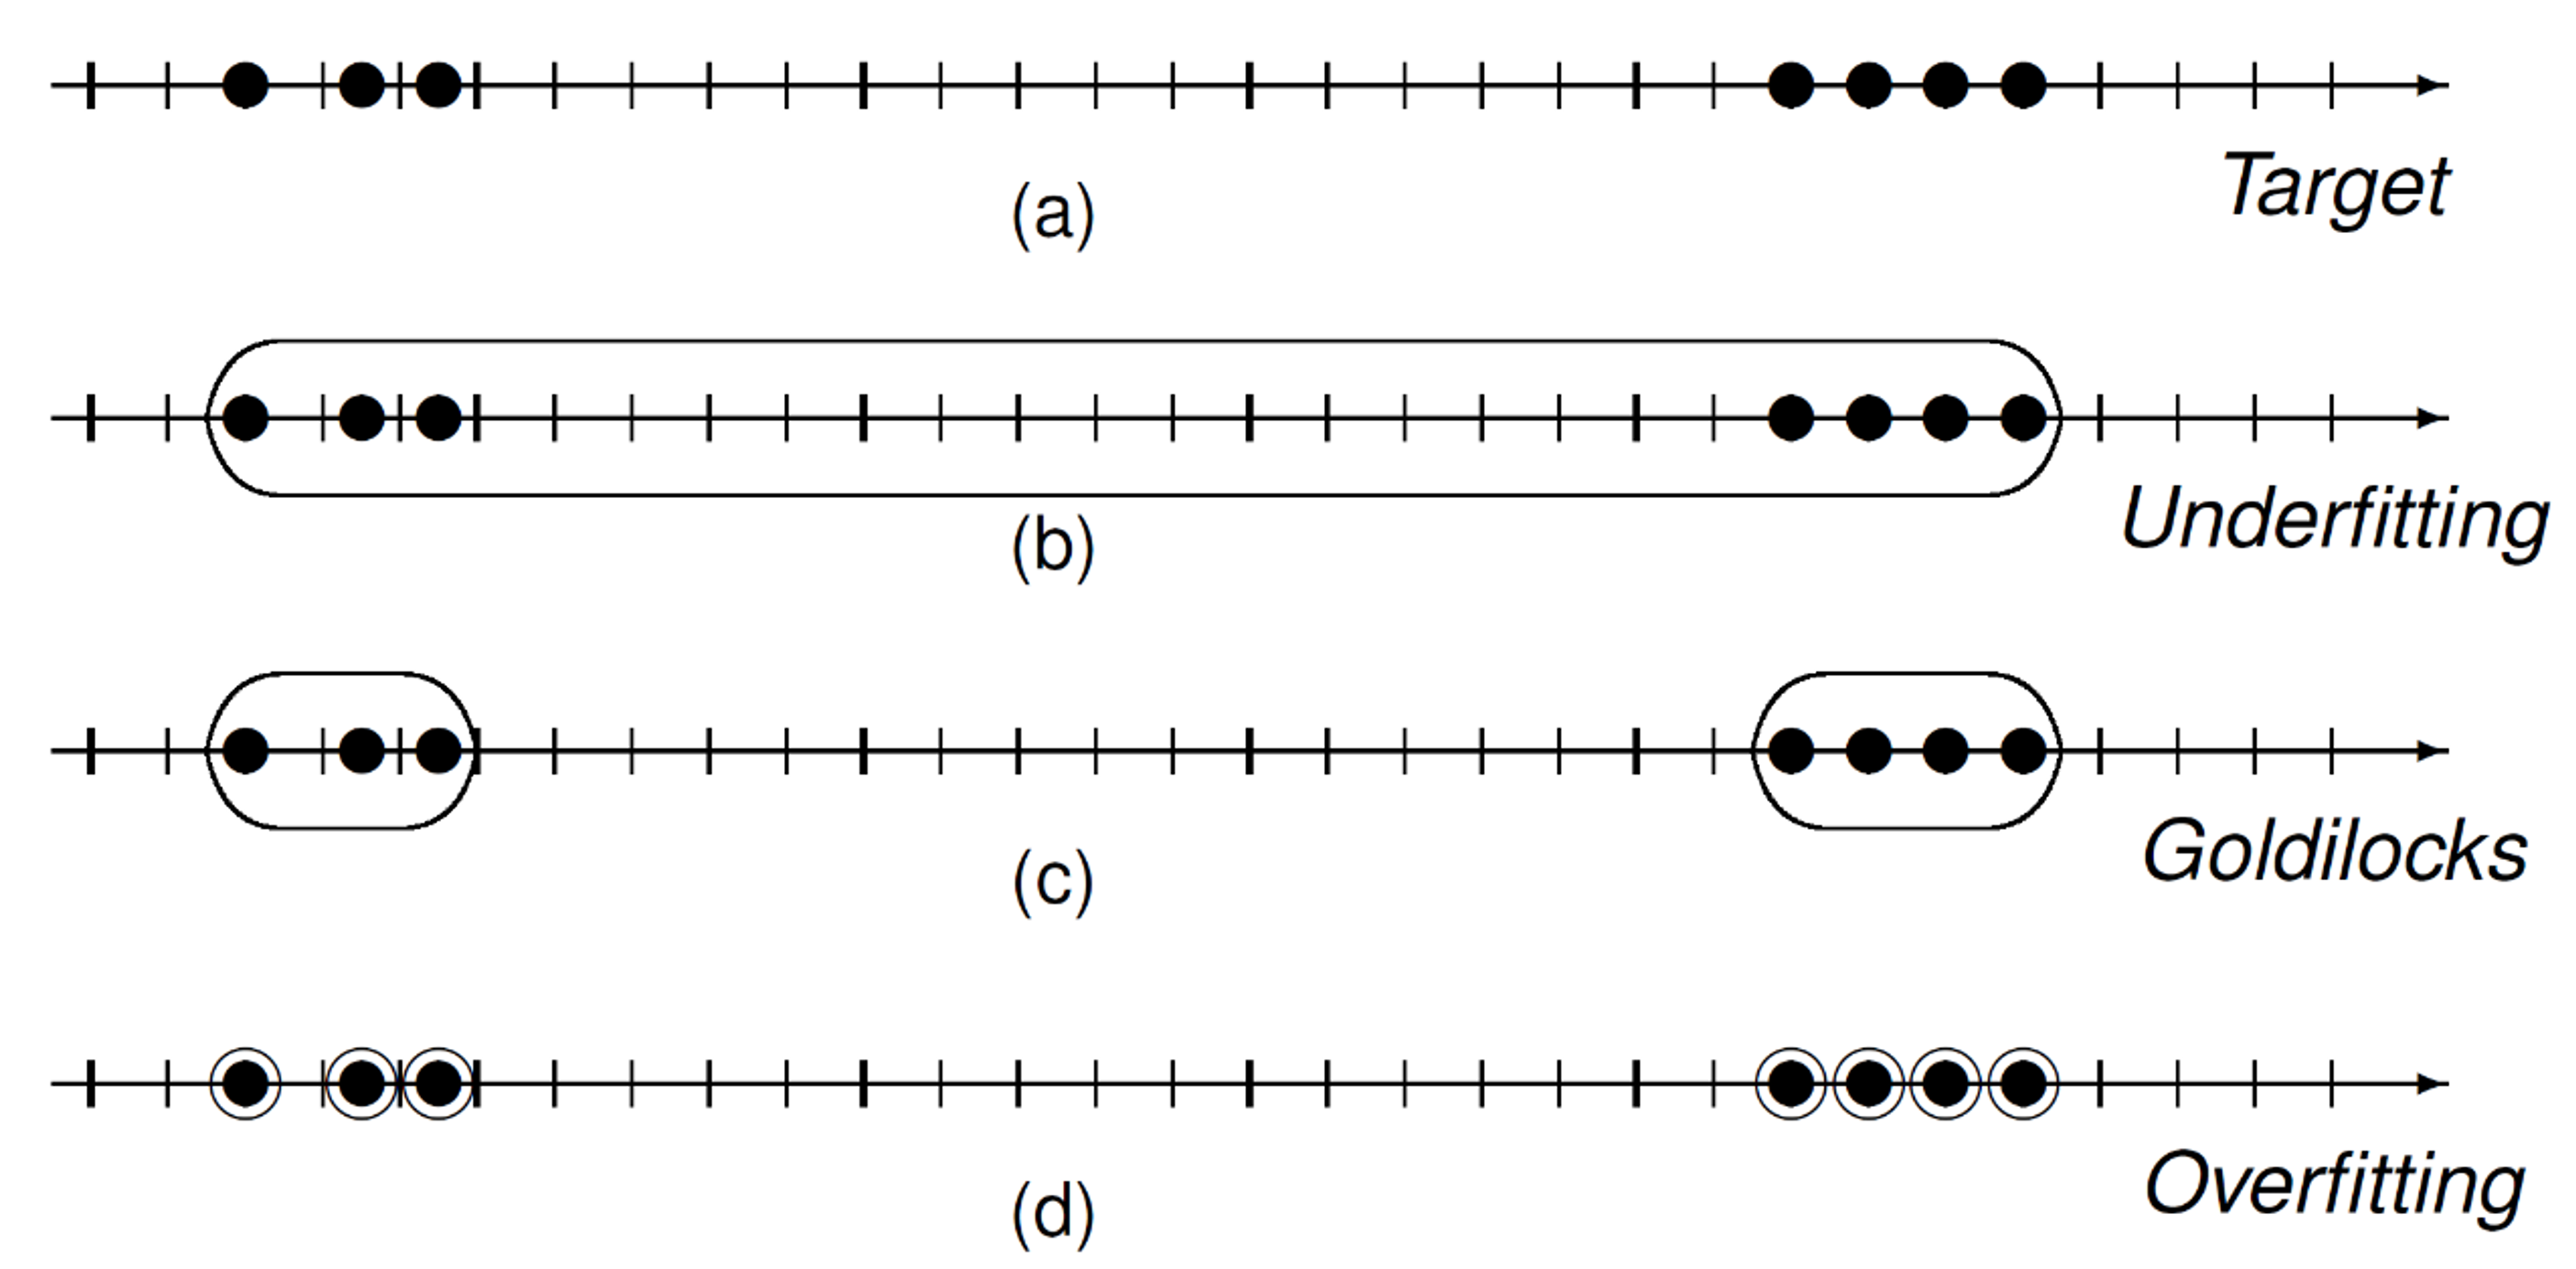
\includegraphics[width=0.5\textwidth]{assets/trees/cont/target_overunder.png}
  \caption{Over- and underfitting in continuous target feature classification}
  \label{fig:3_overunder_target}
\end{figure}

The \textbf{predicted value}, so the output of the decision tree, is the \textbf{average} value within a (leaf) node.


To be able to still use the ID3-algorithm, the decision for $\mathbf{d}[best]$ needs to be adjusted.
\begin{itemize}
  \item Instead of $\mathbf{d}[best] \leftarrow \arg\max_{d\in\mathbf{d}} IG(d, \mathcal{D})$, we will
  \item Base the split on the feature lowering the weighted variance within the subtrees as much as possible, so $\mathbf{b}[best] \leftarrow \arg\min_{d\in\mathbf{d}}\sum_{l\in levels(d)}\frac{|\mathcal{D}_{d=l}|}{|\mathcal{D}|}\cdot var(t, \mathcal{D}_{d=;})$
\end{itemize}
In general, there are some extensions of ID3 implementing different ideas presented throughout this chapter:
\begin{itemize}
  \item ID3 is the original.
  \item C4.5 can also deal with continuous features, missing values, implements post-pruning, etc. (C5.0 extends this further)
  \item J48 is an open-source implementation of C4.5.
  \item CART (classification and regression trees) use the Gini index, can handle continuous features, and can deal with missing values.
  \item CAID (Chi-square automatic interaction detector) relies on the Chi-square test to determine the best next split at each stop.
\end{itemize}


